\begin{figure}[bt!]
	\begin{center}
		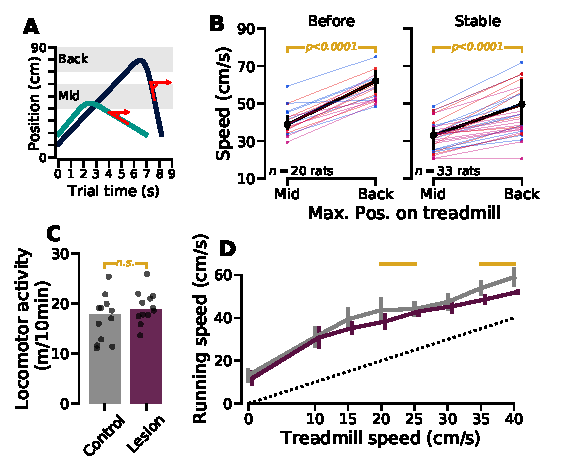
\includegraphics[scale=1]{ch-lesion/figures/MotorPreserved.pdf}
		\caption[Preserved Motor Control After Striatal Lesion]
		{\textbf{Preserved spontaneous locomotor activity and modulation of running speed following striatal lesion.}
		\textbf{A)}
		Displacement while exploring a new (and immobile) treadmill for non-lesioned (control, $n=12$) and lesioned rats ($n=12$, same color code for individual lesion type as in \autoref{fig:lesion:task}).
		\textbf{B)}
		Average running speed in a free running task (no reward) in which control and lesioned rats were submitted to trials with incremental treadmill speed (same color code as in panel~A, see \autoref{ch:methods:loco}).
		Golden lines indicate significant differences between groups (corrected for multiple comparisons).
		\textbf{C)}
		Trials were split into 2~categories depending on whether rats initiated their run from the middle or back portion of the treadmill.
		Speed was computed and averaged across trial type for sessions with stable performance.
		\textbf{D)}
		Speed of the runs initiated from either the middle or back portion of the treadmill, and calculated for each animal over the last 5~sessions before lesion (\textit{left}) and the last 5~stable sessions after lesion (\textit{right}).
		}
		\label{fig:lesion:motorOk}
	\end{center}
\end{figure}